
  Real time collaboration applications have become a huge help on team tasks, providing a great boost on business, research and investigation velocity. Technologies like this are appearing along this days, but they couln't be possible years ago because technology was limited or unavailable. Although todays technology is limited on some aspects, we are doing progress in order to improve the web ecosystem, by creating standards and migrating to newer technologies.

  Our first concern on real time collaboration applications, besides the communication itself, is the data storage and representation. Because most browsers are recommended to limit local storage to at least five megabytes per origin, storing multimedia content is not a viable solution.

  If, for instance, one whants to rewind a real time video, recordings will be needed from who is streaming the video. 

  \ac{RTP}\footnote{rfc3550} is used for streaming audio and video over \ac{IP}, the multimedia content is transported on the payload of \ac{RTP} messages, \ac{RTP} contains headers for payload indentification. \ac{RTP} is independent from its payload type, allowing to transport any kind of encoded multimedia. A sequence number is used for sorting received packets.

  \ac{RTP} allows to change its requirements and add extensions to it with profiles, one of the most used is the \ac{RTP} profile for audio and video \footnote{rfc3551} which lists the payload encodings and compression algorithms. This profile also assigns a name to each encoding which may be used other protocols like \ac{SDP}.

  \ac{RTP} recorders are independent of payload encoding, they don't decode \ac{RTP} packets, they record packets instead, allowing to record all video and audio formats.

\begin{figure}[H]
	\begin{center}
		\centering
		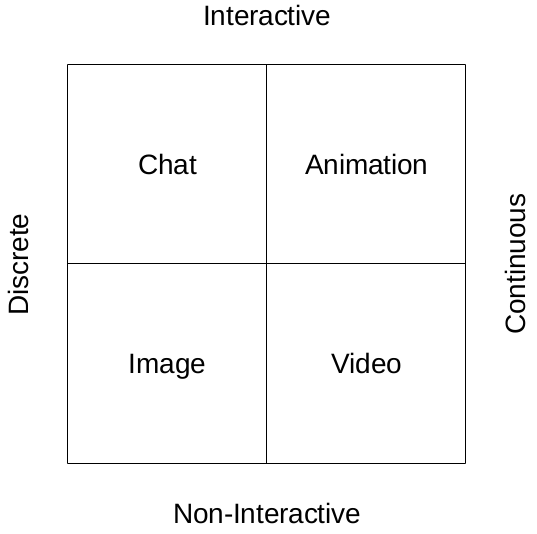
\includegraphics[width=0.35\textwidth]{figures/media_types.png}

	\caption{Media Types}
	\end{center}
\end{figure}

	Media Types can be described as discrete or continuos and interactive or non-interactive. For example an image is non-interctive and discrete, for instance, a video is continuos and non-interactive. A simple chat with just text is interactive and discrete. An animation that changes in function of user behaviour is interactive and continuous.

	Streaming protocols like \ac {RTP} were designed for continuous and non-interactive media types, such as audio and video. Discrete and non-interactive media don't need to streamed through \ac{RTP} because they don't change with. For example if an image appears in a specific time interval, just the \ac{HTML} or javascript that will reference the image must be streamed, the image itself is then transfered through \ac{HTTP}.

	In order to play any kind of stream, a player for interactive stream is needed downloading an environment, decoding the \ac{RTP} payload to determine the state and display it to the user. Streaming interactive media like the combination of \ac{HTML}, \ac{CSS} and JavaScript requires more than interpreting the code, a streamed user interface may contain an internal state that is not shown on code.

	Everytime an event is proccessed on one of the endpoints, both sender and receivers state must stay synchronized, otherwise events may behave differently.

	To achieve synchronization of interactive data most packets have three types: State, Delta-State and Event. State packet defines environment's complete state. Delta-State packets tranports just the piece of state that changed. Event packets informs that an event ocurred over the interactive media. 

	An \ac{RTP} recorder can have two operation modes, recording or playback. Traditional \ac{RTP} players can do random access, in contrast, interactive \ac{RTP} players must restore the environment and context at a given time. The environment is the initial state, so we can call it a non-interactive descrete media and handle it over \ac{HTTP}. After the receiver has received the environment, it should calculate the state at the given time. 

	If the \ac{RTP} recorder controls the correct data to send to the receivers, it cannot be a simple \ac{RTP} recorder as it must compute the state or delta-state to send. Therefore, if the receiver receives all recorded packets, it can calculate the current state from a nearest complete state. Having too much complete states, results on more precise random accesses but there is the storage space payback. On the other hand if there are few complete states recorded followed by delta-states, the recorded stream will occupy less storage space, but random accesses will be less granular.

	By recording and streaming the interactive media's complete state periodically, it is possible to restore the media state even if messages are lost.

	With such an interactive \ac{RTP} recorder it is then possible to record, play, fast forward, fast rewind, stop and jump to random positions.

  \cite{interactive_stream} proposed an \ac{RTP} profile for real-time transmission of interactive media. This new profile reuses much of video and audio profile implementation, integrating the interactive component.
	
  {\color{red}[Model View Controller (Suited for interactive RTP)]}


  {\color{red}[Identity]}



\quote{There is strong growth in the deployment of devices that integrate regular Web technologies such as HTML, CSS, and SVG, coupled with various device APIs.}